\documentclass[border=16pt]{standalone}
\usepackage{tikz}
\usetikzlibrary{arrows.meta, positioning}
\begin{document}
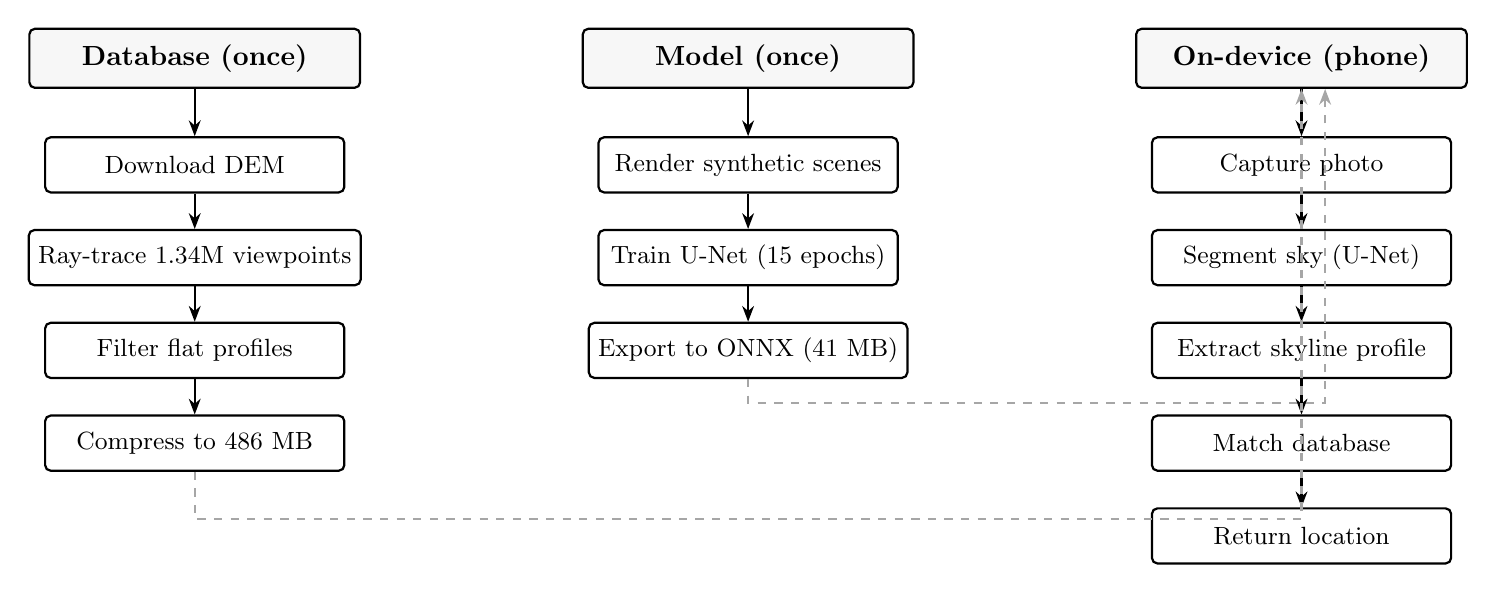
\begin{tikzpicture}[
    node distance=0.55cm and 0.8cm,
    stage/.style={rectangle, draw=black, thick, minimum width=4.2cm, minimum height=0.75cm,
                  text centered, font=\normalsize\bfseries, fill=gray!6, rounded corners=2pt},
    box/.style={rectangle, draw=black, thick, minimum width=3.8cm, minimum height=0.7cm,
                text centered, font=\small, rounded corners=2pt},
    arr/.style={-{Stealth[length=2mm]}, thick},
    arrgray/.style={-{Stealth[length=2mm]}, thick, gray!70},
]

% ── Column 1: Database (done once) ──
\node[stage] (db) {Database (once)};
\node[box, below=0.6cm of db] (db1) {Download DEM};
\node[box, below=0.45cm of db1] (db2) {Ray-trace 1.34M viewpoints};
\node[box, below=0.45cm of db2] (db3) {Filter flat profiles};
\node[box, below=0.45cm of db3] (db4) {Compress to 486 MB};

\draw[arr] (db) -- (db1);
\draw[arr] (db1) -- (db2);
\draw[arr] (db2) -- (db3);
\draw[arr] (db3) -- (db4);

% ── Column 2: Model training (done once) ──
\node[stage, right=2.8cm of db] (mdl) {Model (once)};
\node[box, below=0.6cm of mdl] (m1) {Render synthetic scenes};
\node[box, below=0.45cm of m1] (m2) {Train U-Net (15 epochs)};
\node[box, below=0.45cm of m2] (m3) {Export to ONNX (41 MB)};

\draw[arr] (mdl) -- (m1);
\draw[arr] (m1) -- (m2);
\draw[arr] (m2) -- (m3);

% ── Column 3: On-device (runs on phone) ──
\node[stage, right=2.8cm of mdl] (dev) {On-device (phone)};
\node[box, below=0.6cm of dev] (d1) {Capture photo};
\node[box, below=0.45cm of d1] (d2) {Segment sky (U-Net)};
\node[box, below=0.45cm of d2] (d3) {Extract skyline profile};
\node[box, below=0.45cm of d3] (d4) {Match database};
\node[box, below=0.45cm of d4] (d5) {Return location};

\draw[arr] (dev) -- (d1);
\draw[arr] (d1) -- (d2);
\draw[arr] (d2) -- (d3);
\draw[arr] (d3) -- (d4);
\draw[arr] (d4) -- (d5);

% ── Cross-column arrows (routed below boxes to avoid crossing) ──
\draw[arrgray, dashed] (db4.south) -- ++(0,-0.6) -| (dev.south);
\draw[arrgray, dashed] (m3.south) -- ++(0,-0.3) -| ([xshift=0.3cm]dev.south);

\end{tikzpicture}
\end{document}
